\documentclass[11pt,a4paper]{article}
\usepackage[T1]{fontenc}
\usepackage{lmodern}
\usepackage[margin=2.3cm]{geometry}
\usepackage{microtype}
\usepackage{amsmath,amssymb}
\usepackage{graphicx}
\usepackage{booktabs,tabularx,array,multirow}
\usepackage{caption,subcaption}
\usepackage{float}
\usepackage{xcolor}
\usepackage{listings}
\usepackage{enumitem}
\usepackage{fancyhdr}
\usepackage{titlesec}
\usepackage[colorlinks=true,linkcolor={blue!55!black},urlcolor={blue!55!black},citecolor={blue!55!black}]{hyperref}
\usepackage[capitalise,noabbrev]{cleveref}

\graphicspath{{figures/}{../RESULTS/}}
% generated by make_numbers.py -- do not edit
\newcommand{\HiSigA}{0.268345(48)}
\newcommand{\HiAA}{0.23682(17)}
\newcommand{\HiSigB}{0.268351(46)}
\newcommand{\HiAB}{0.23757(17)}
\newcommand{\HiSigC}{0.268354(44)}
\newcommand{\HiAC}{0.23730(16)}
\newcommand{\HiSlope}{$-0.00023\pm0.00012$}
\newcommand{\HiAav}{0.23724(10)}
\newcommand{\HiAmav}{0.23722(10)}
\newcommand{\HiAvav}{0.26651(9)}


\definecolor{codebg}{HTML}{F6F6F4}
\definecolor{codefr}{HTML}{D9D8D3}
\lstdefinestyle{fortran}{language=[77]Fortran,basicstyle=\ttfamily\footnotesize,
  backgroundcolor=\color{codebg},frame=single,rulecolor=\color{codefr},framesep=4pt,
  xleftmargin=6pt,xrightmargin=6pt,columns=fullflexible,keepspaces=true,
  keywordstyle=\bfseries,commentstyle=\itshape\color{black!60},showstringspaces=false,
  escapeinside={(*@}{@*)}}
\lstset{style=fortran}
\newcommand{\code}[1]{\texttt{#1}}
\newcommand{\phok}{PHOKHARA}
\newcommand{\ceex}{CEEX}
\newcommand{\bby}{BabaYaga}
\newcommand{\gosam}{GoSam}
\newcommand{\Ath}{A(\theta^+)}

\pagestyle{fancy}\fancyhf{}
\lhead{\small CEEX vs PHOKHARA -- KLOE-LA $\pi^+\pi^-\gamma$ at NLO}
\rhead{\small\thepage}
\renewcommand{\headrulewidth}{0.4pt}
\titleformat{\section}{\large\bfseries}{\thesection}{0.8em}{}
\titleformat{\subsection}{\normalsize\bfseries}{\thesubsection}{0.8em}{}
\setlist{itemsep=2pt,topsep=4pt}
\captionsetup{font=small,labelfont=bf}
\setlength{\emergencystretch}{2em}

\title{\vspace{-1.2cm}\textbf{Origin of the \ceex--\phok{} discrepancy in the pion angular
  distributions}\\[4pt]\large KLOE large-angle scenario, $e^+e^-\to\pi^+\pi^-\gamma$ at NLO,
  $F_\pi=1$, no vacuum polarisation}
\author{Jeremy Paltrinieri\thanks{Analysis carried out with Claude Code (Anthropic).
  Repository: \url{https://github.com/jpaltrinieri/CEEX_PHOKHARA_ANALYSIS}}}
\date{23 September 2026}

\begin{document}
\maketitle
\thispagestyle{fancy}

\begin{abstract}\noindent
In the KLOE large-angle (KLOE-LA) scenario the NLO predictions of \ceex{} and \phok{}~10.0
for $e^+e^-\to\pi^+\pi^-\gamma$ agree in the total cross section and in every charge-even
distribution, but disagree in the pion polar angles: the forward--backward asymmetry of the
$\pi^+$ is $\Ath=0.2375$ in \ceex{} (and $0.2372$ in \bby) against $0.2787$ in \phok.
We show that the difference is entirely due to two errors in the one-photon ISR$\times$FSR
interference at NLO in \phok{} (routine \code{ampLO}, pion branch of the full-NLO mode): a
misplaced parenthesis that adds three helicity terms of the tree interference a second time,
and a block that keeps the tree interference together with an analytic ISR soft function that
the full-NLO mode replaces by the eikonal elsewhere. The second error makes the \phok{}
asymmetry depend on the unphysical soft-photon cutoff. A point-by-point comparison of the
one-photon matrix elements shows that the two errors account for the whole charge-odd
difference to $2.5\times10^{-5}$ of the tree. With both corrected, \phok{} gives
$\Ath=\HiAav$, independent of the cutoff and in agreement with \ceex{} and \bby.
\end{abstract}

\setcounter{tocdepth}{1}
\tableofcontents
\vspace{0.4cm}

%=========================================================================================
\section{Summary of findings}
\label{sec:summary}

\begin{enumerate}[label=\arabic*.,leftmargin=*]
\item \textbf{The disagreement is reproduced} with a fresh \phok{} build and fresh \ceex{} runs
  (\cref{sec:discrepancy}): totals agree to $10^{-4}$, charge-even shapes agree, and only
  $\theta^\pm$ and $\theta_{\rm avg}$ differ ($\chi^2/{\rm ndf}\approx 10^3$). At LO the two
  codes agree exactly.
\item \textbf{The \phok{} asymmetry depends on the soft cutoff $w$}: $\Ath$ changes by
  $+0.0156$ per decade of $w$ while $\sigma$ is constant (\cref{sec:t1}).
\item \textbf{The whole effect sits in the charge-odd part of the one-photon contribution}
  (Born + virtual + soft); the hard two-photon emission agrees between the codes
  (\cref{sec:t3}).
\item \textbf{Two errors in \phok{} explain it point by point} (\cref{sec:t4,sec:bugs}):
  \begin{itemize}
  \item \textbf{H1} -- \code{phokhara\_10.0.f:9969--9982}: the factor $(v_f+v_s)$ multiplies only
    the last of four helicity terms of the tree interference;
  \item \textbf{H2} -- block B5, the ISR one-loop current times the FSR tree
    (\code{phokhara\_10.0.f:9998--10007}; \code{ISRcurrent\_no\_mass\_terms.f:134,210}):
    an extra ${\rm Re}[F^*I]\,(1+S_{\rm ISR}(w))$.
  \end{itemize}
  Subtracting both leaves a per-point residual of $2.5\times10^{-5}$ of the tree.
\item \textbf{With both corrected}, $\Ath$ no longer depends on $w$ and agrees with \ceex{} and
  \bby{} (\cref{sec:fix}). Totals and charge-even distributions are unchanged.
\end{enumerate}

%=========================================================================================
\section{Setup}
\label{sec:setup}

\paragraph{Scenario.} KLOE-LA (Strong2020 KLOE-I), $\sqrt s=1.02$~GeV:
$50^\circ\le\theta_\pm\le130^\circ$; $|p^z_\pm|>90$~MeV or $p^\perp_\pm>160$~MeV; at least one
photon with $50^\circ\le\theta_\gamma\le130^\circ$ and $E_\gamma>20$~MeV;
$0.1\le M_{\pi\pi}^2\le0.85$~GeV$^2$. Angles are measured from the electron beam in both codes.
Histograms: the 18 KLOE-I observables with 600 uniform bins. The forward--backward asymmetry is
$A=[\sigma(\theta<90^\circ)-\sigma(\theta>90^\circ)]/\sigma$.

\paragraph{Codes.}
\begin{itemize}
\item \textbf{\ceex-main} (commit \code{e05d007}): \code{pipig --scenario=KLOE-LA --NLO}, one-loop
  amplitudes from \gosam{} (\code{eepipig\_noVP\_1L\_onshell}, \code{eepipigg}), YFS soft
  subtraction with cutoff $E_{\min}=10^{-4}$ or $10^{-5}$~GeV; 5 MPI ranks per task.
\item \textbf{\phok~10.0} (\code{PHOKARA\_10.0} @ \code{133d68b}) with the KLOE-I cut file,
  card \code{nlo=nlo2=1}, IFSNLO$=1$, ISR+INT+FSR, \code{ivac=0}, \code{FF\_pion=-1} ($F_\pi=1$),
  no GVMD, no $f_0$, soft cutoff $w=10^{-5}$ (soft region $E_\gamma<w\sqrt s$). The production
  binary \code{phokhara\_nostop} only disables the abort on ``Max(i) too small''
  (\cref{sec:other}); only weighted events are used.
\item \textbf{\bby} and the earlier \phok{} reference set (5~Aug) are taken from the Strong2020
  comparison files.
\end{itemize}

\paragraph{Pipeline.} SLURM arrays per run name; \ceex{} rank outputs are screened with
\code{check\_total.sh} and outliers are moved aside (\code{quarantine.sh}) before merging;
\code{plot\_compare.py} produces the distribution and ratio plots. Everything is in the
repository (\cref{app:files}).

%=========================================================================================
\section{The discrepancy}
\label{sec:discrepancy}

\begin{table}[H]
\centering\small
\caption{Production runs (prod500k): \phok{} 300 seeds $\times$ 500k events; \ceex{} 59 tasks
$\times$ 5 ranks $\times$ 500k per $E_{\min}$ (one slow task cancelled, one outlier rank excluded).}
\label{tab:prod}
\begin{tabular}{lcc}
\toprule
 & $\sigma$ [nb] & $\Ath$ \\
\midrule
\ceex, $E_{\min}=10^{-4}$ GeV & 0.26840(4) & 0.23751(13) \\
\ceex, $E_{\min}=10^{-5}$ GeV & 0.26836(4) & 0.23752(14) \\
\bby & 0.268389(4) & 0.23724(1) \\
\phok, this work & 0.268353(46) & 0.27872(16) \\
\phok, earlier reference & 0.268393(23) & 0.27861(8) \\
\bottomrule
\end{tabular}
\end{table}

The new \phok{} run reproduces the earlier reference. All generators pass the
charge-conjugation mirror test $\theta^+(\theta)=\theta^-(180^\circ-\theta)$, so this is not a
mislabelled charge. \Cref{fig:before} shows the $\theta^+$ distribution and \cref{fig:before-ov} the ratio of every
observable to \phok: only the three pion angles are off, by a smooth tilt from $0.95$ to $1.28$.

\begin{figure}[H]
\centering

\includegraphics[width=0.62\textwidth]{prod500k/60bins/pi_kloe_la_lth+.pdf}
\caption{\textbf{Before the fix} (prod500k): $d\sigma/d\theta^+$, \ceex/\bby, and \ceex{} and
\bby{} over \phok{} (60 bins). \ceex{} (black, grey) and \bby{} (blue) agree; \phok{} (red) is
tilted.}
\label{fig:before}
\end{figure}

\begin{figure}[H]
\centering

\includegraphics[width=\textwidth]{prod500k/60bins/overview_vs_phokhara.pdf}
\caption{\textbf{Before the fix}: every observable, \ceex{} and \bby{} over \phok. Only
$\theta^+$, $\theta^-$ and $\theta_{\rm avg}$ are off; the spikes in $M_{\pi\pi\gamma}$ and
$M_{\rm trk}$ are empty tail bins.}
\label{fig:before-ov}
\end{figure}

At LO the codes agree exactly (earlier runs with the Strong2020 form factor:
$A_{\rm LO}=0.0779$ and $\sigma_{\rm LO}=2.6523$~nb in both), so the difference lies in the NLO
correction to the charge-odd part of the cross section.

%=========================================================================================
\section{Strategy}
\label{sec:strategy}

The difference is charge-odd ($C$-odd): it flips sign under $\pi^+\leftrightarrow\pi^-$ and
integrates to zero over the symmetric cuts. At $\mathcal O(\alpha^4)$ the $C$-odd part of the
cross section consists of the gauge-invariant classes $Q_e^5Q_\pi^3$ and $Q_e^3Q_\pi^5$ (the tree
interference is $Q_e^3Q_\pi^3$). Three tools were used to isolate it:
\begin{itemize}
\item \textbf{Cutoff independence.} The split into one-photon (Born + virtual + soft photons
  below the cutoff) and two-photon (hard) parts depends on the cutoff; the sum must not.
\item \textbf{Matched split.} For the same cutoff each part is uniquely defined, so the two codes
  must agree part by part. \phok{} $w=9.804\times10^{-6}$ ($w\sqrt s=10^{-5}$~GeV) matches
  \ceex{} $E_{\min}=10^{-5}$~GeV.
\item \textbf{Momentum swap.} At a phase-space point, the $C$-odd part of any piece $X$ is
  $X_{\rm odd}=\tfrac12[X(p_+,p_-)-X(p_-,p_+)]$. No charge parameter is needed.
\end{itemize}
Each histogram-level test used enough statistics to resolve $\Ath$ to $\sim10^{-3}$ while
checking that $\sigma$ and $M_{\pi\pi}$ are unchanged. The plan with all tests and hypotheses
is in \code{plan.txt}.

%=========================================================================================
\section{Tests}
\label{sec:tests}

\subsection{T1: soft-cutoff scan}
\label{sec:t1}
\begin{table}[H]
\centering\small
\caption{Unpatched \phok, 30 seeds $\times$ 100k per value of $w$.}
\label{tab:t1}
\begin{tabular}{lcccc}
\toprule
$w$ & $10^{-3}$ & $10^{-4}$ & $10^{-5}$ & $10^{-6}$ \\
\midrule
$\sigma_{1\gamma}$ [nb] & 0.1386 & 0.0955 & 0.0530 & 0.0103 \\
$\sigma_{2\gamma}$ [nb] & 0.1297 & 0.1728 & 0.2149 & 0.2580 \\
$\sigma$ [nb] & 0.26833(33) & 0.26827(35) & 0.26792(33) & 0.26830(30) \\
$\Ath$ & 0.3106(11) & 0.2950(12) & 0.2785(12) & 0.2637(11) \\
\bottomrule
\end{tabular}
\end{table}
$\Ath$ falls linearly in $\ln w$, by $0.0156$ per decade, while $\sigma$ is constant to
$0.1\%$: the charge-even soft logarithms cancel between the one- and two-photon parts, a
charge-odd one does not. In \ceex{}, $E_{\min}=10^{-4}$ and $10^{-5}$~GeV give the same $\Ath$
to $10^{-4}$.

\subsection{T2: diagnostic variants}
\label{sec:t2}
Three diagnostic \phok{} builds were run at $w=10^{-4},10^{-5},10^{-6}$ (\cref{fig:wscan}a):
\begin{itemize}
\item \textbf{H1 fixed} (the parenthesis of \cref{sec:h1}): $\Ath$ moves by $-0.037$ and keeps
  its slope. H1 is a $w$-independent error.
\item \textbf{B5 soft log removed} (probe): $\Ath$ becomes flat in $w$, but at $0.355$. The whole
  $w$-dependence comes from this term; removing only the logarithm is not the right correction.
\item \textbf{Both}: flat, at $0.319$.
\end{itemize}

\begin{figure}[H]
\centering
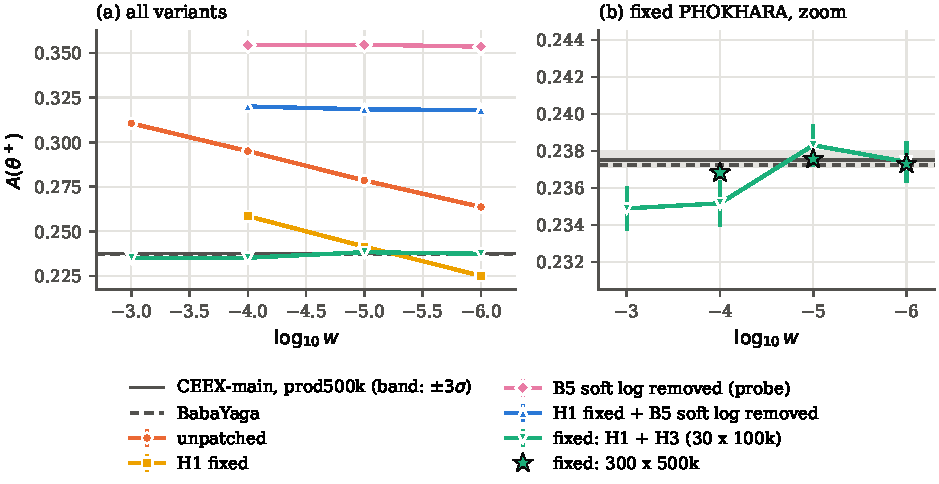
\includegraphics[width=0.96\textwidth]{fig_wscan.pdf}
\caption{$\Ath$ against the \phok{} soft cutoff for the unpatched code, the T2 diagnostic
variants and the fixed code (H1 + H3), with \ceex{} (grey band: $\pm3\sigma$) and \bby. The zoom
(b) shows the fixed code at 30$\times$100k and at 300$\times$500k (stars).}
\label{fig:wscan}
\end{figure}

\subsection{T3: split by photon multiplicity}
\label{sec:t3}
\ceex-main was given an opt-in output of the per-multiplicity histograms
(\code{CEEX\_NPH\_HISTOS=1}); \phok{} writes them with \code{print\_summed=1}.
\begin{table}[H]
\centering\small
\caption{Matched cutoff ($10^{-5}$ GeV). \ceex{} 10 seeds $\times$ 5 ranks $\times$ 100k; \phok{} 30 $\times$ 100k (unpatched).}
\label{tab:t3}
\begin{tabular}{lccccc}
\toprule
 & \multicolumn{2}{c}{$\sigma$ [nb]} & \multicolumn{2}{c}{$\Ath$} & angle shapes \\
 & \ceex & \phok & \ceex & \phok & $\chi^2/{\rm ndf}$ \\
\midrule
1 photon (Born+V+S) & 0.05268(7) & 0.05239(24) & 0.0375(13) & 0.2360(44) & 79--94 \\
2 photons (hard) & 0.21560(37) & 0.21588(23) & 0.2901(16) & 0.2855(10) & 1.0--1.4 \\
\bottomrule
\end{tabular}
\end{table}
The one-photon parts have the same $\sigma$ and the same $M_{\pi\pi}$, $\theta_\gamma$ and
$E_\gamma$ shapes, but charge-odd cross sections of $0.0020$ (\ceex) and $0.0124$~nb (\phok). The
difference, $0.0104$~nb, is the whole total discrepancy (\cref{fig:t3}). The hard two-photon
parts agree.

\begin{figure}[H]
\centering
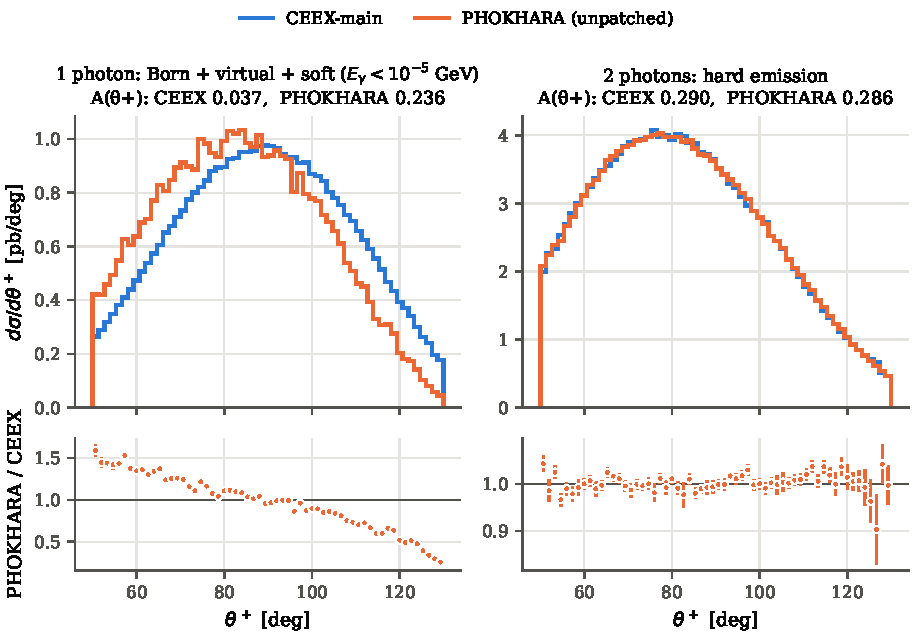
\includegraphics[width=0.85\textwidth]{fig_t3.pdf}
\caption{T3: $d\sigma/d\theta^+$ of the one-photon (left) and two-photon (right) contributions at a
matched cutoff, with the ratio \phok/\ceex.}
\label{fig:t3}
\end{figure}

\subsection{T4: point-by-point comparison}
\label{sec:t4}
988 accepted one-photon KLOE-LA points were dumped by a \phok{} variant
(\code{phokhara\_dump}) together with every piece of the one-photon matrix element, at the event
and with the pion momenta swapped. A \ceex-main driver (\code{t4\_ceex}) evaluates the tree, the
hard virtual $\frac{\alpha}{4\pi}D$ (\gosam{} finite part plus mass counterterm), the
wave-function counterterm and the YFS factor at the same momenta; the pion mass is set to
\phok's value. Each code is normalised to its own charge-even tree:
\begin{itemize}
\item tree $C$-odd/$C$-even ratio: identical to $7\times10^{-13}$;
\item $C$-even NLO correction: \ceex{} $-0.77566$, \phok{} $-0.77570$, per-point difference rms $10^{-5}$;
\item $C$-odd NLO correction: per-point difference $D$ with rms $0.099$;
\item $C$-odd soft (eikonal/YFS) part: agrees, rms $7\times10^{-4}$.
\end{itemize}
$D$ is exactly proportional to the tree interference at every point. Subtracting the two errors,
each computed exactly per point ($v_s=0.29655$, $v_f=0.023$--$0.036$,
$S_{\rm ISR}(w)=-0.95556$),
\[
  \text{pred}_{\rm H1}=B_4-\tfrac12B_3\,(v_f+v_s),\qquad
  \text{pred}_{\rm H2}=\tfrac12B_3\,(1+S_{\rm ISR}(w)),
\]
leaves a residual of rms $2.5\times10^{-5}$ with mean $10^{-6}$ (\cref{fig:t4}). H1 alone leaves
$1.2\times10^{-2}$, H2 alone $8.8\times10^{-2}$.

\begin{figure}[H]
\centering
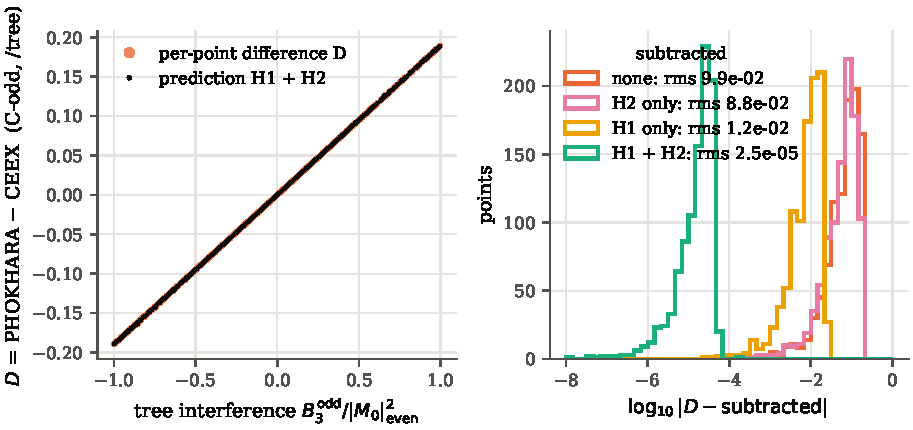
\includegraphics[width=0.95\textwidth]{fig_t4.pdf}
\caption{T4, 988 points. Left: the $C$-odd difference $D$ against the tree interference, with the
H1+H2 prediction. Right: $\log_{10}|D-\text{subtracted}|$ for no subtraction, H1, H2 and H1+H2.}
\label{fig:t4}
\end{figure}

%=========================================================================================
\section{The two errors in \phok}
\label{sec:bugs}

The one-photon weight in the full-NLO mode is
$\code{amplit}+\code{helicityampLO}+\code{NLOpions}+\code{virt\_pions}$. In \code{ampLO} (inside
\code{helicityampLO}) the pion branch adds, per photon polarisation: B1 $=|F|^2(1+v_s)$,
B2 $=|I|^2v_f$, B3 $=2{\rm Re}[I^*F]$ (tree interference), B4 and B5 below. Here $I$ and $F$ are
the ISR and FSR tree amplitudes, $v_s$ the electron-vertex correction at $s$ and $v_f$ the
pion-vertex correction at $q^2$, both $|M|^2$-level factors with the analytic soft part removed.

\subsection{\texorpdfstring{H1: misplaced factor in the ISR$\times$FSR correction}{H1: misplaced factor in the ISR x FSR correction}}
\label{sec:h1}
\begin{lstlisting}
      if((nlo2.eq.1).and.(pion.eq.1))then
         ampLO = ampLO
     4     + dreal(
     5         dconjg(dme*(mb(1,1)-ma(1,1))*cvac_qq)*dme*(ddpl(1,1)-ddmi(1,1))*cvac_s   ! T1
     6       + dconjg(dme*(mb(2,2)-ma(2,2))*cvac_qq)*dme*(ddpl(2,2)-ddmi(2,2))*cvac_s   ! T2
     7       + dconjg((-ebppb*ma(2,1)+el_m2/ebppb*mb(2,1))*cvac_qq)
     8           *(-ebppb*ddmi(2,1)+el_m2/ebppb*ddpl(2,1))*cvac_s                       ! T3
     9       + dconjg((ebppb*mb(1,2)-el_m2/ebppb*ma(1,2))*cvac_qq)
     1           *(ebppb*ddpl(1,2)-el_m2/ebppb*ddmi(1,2))*cvac_s                        ! T4
     2           *(ver_f+ver_s) )       (*@\textbf{! multiplies T4 only}@*)
\end{lstlisting}
(Continuation lines re-indented for reading; the code is unchanged.)
The block is meant to be ${\rm Re}[T_1+T_2+T_3+T_4]\,(v_f+v_s)$, the amplitude-level corrections on
each side of $2{\rm Re}[I^*F]$. As written it is
${\rm Re}[T_1+T_2+T_3]+{\rm Re}[T_4](v_f+v_s)$, so ${\rm Re}[T_1+T_2+T_3]$ (about a third of the
tree interference) is added with coefficient 1. The muon version of the same block
(\code{phokhara\_10.0.f:10384--10394}) is correct:
\code{2*dreal(sum)*(ver\_s+ver\_f)/2}.

\textbf{Fix} (\code{variants/h1.patch}): \code{*cvac\_s *(ver\_f+ver\_s) )} $\to$
\code{*cvac\_s )*(ver\_f+ver\_s)}.

\subsection{H2: tree and analytic ISR soft function in the ISR one-loop block}
\label{sec:h2}
Block B5 contracts the FSR tree with the ISR current at one loop:
\begin{lstlisting}
      ampLO=ampLO+dreal( dconjg(... ddpl, ddmi ...)*( ... apl, ami ...) )    ! B5
\end{lstlisting}
The current (\code{hard\_soft\_part/ISRcurrent\_no\_mass\_terms.f}) has the coefficient
\begin{lstlisting}
      V1(1)=2.d0*log(4.d0*w**2)*(log(m2)+1.d0) -4.d0*log(qq2)+3.d0*log(m2) + ...   ! l.134
      V1(1)=(1.d0-2.d0*alpha/4.d0/pi*V1(1))/Sp                                   ! l.210
\end{lstlisting}
It therefore contains the tree (the ``1'') and the analytic ISR soft function, and B5 carries an
extra ${\rm Re}[F^*I]\,(1+S_{\rm ISR}(w))$ with
\[
S_{\rm ISR}(w)=\frac{\alpha}{\pi}\Big[-\ln(4w^2)\,(1+L)-\tfrac12L^2-L-\tfrac{\pi^2}{3}\Big],
\qquad L=\ln\frac{m_e^2}{s}.
\]
\begin{itemize}
\item The tree interference is already added by the \code{fsr=2} block (B3).
\item In the full-NLO mode the analytic ISR soft function is replaced by the eikonal in
  \code{NLOpions}; it is subtracted from $v_s$, $v_f$ and the leptonic tensor, but not here.
\item At $w\simeq10^{-5}$ the two parts nearly cancel ($1+S_{\rm ISR}=0.044$), but
  $S_{\rm ISR}$ changes by $0.152$ per decade of $w$. This gives the T1 slope:
  $\tfrac12\cdot0.152\cdot A_{\rm LO}\approx0.019$ per decade, against $0.0156$ measured.
\end{itemize}
\textbf{Fix} (\code{variants/h3.patch}): subtract ${\rm Re}[\sum T]\,(1+S_{\rm ISR})$ after B5, with
$S_{\rm ISR}$ computed as in the $v_s$ subtraction.

%=========================================================================================
\section{Result with the fix}
\label{sec:fix}
\code{phokhara\_fix} is the production binary with \code{h1.patch} and \code{h3.patch}.
\begin{table}[H]
\centering\small
\caption{Fixed \phok{} against the soft cutoff.}
\label{tab:fix}
\begin{tabular}{lcccc}
\toprule
$w$ & $10^{-3}$ & $10^{-4}$ & $10^{-5}$ & $10^{-6}$ \\
\midrule
\multicolumn{5}{l}{\emph{30 seeds $\times$ 100k}} \\
$\sigma$ [nb] & 0.26799(33) & 0.26892(35) & 0.26854(32) & 0.26784(31) \\
$\Ath$ & 0.2349(12) & 0.2352(13) & 0.2383(12) & 0.2374(11) \\
\multicolumn{5}{l}{\emph{300 seeds $\times$ 500k}} \\
$\sigma$ [nb] & -- & \HiSigA & \HiSigB & \HiSigC \\
$\Ath$ & -- & \HiAA & \HiAB & \HiAC \\
\bottomrule
\end{tabular}
\end{table}
At high statistics the slope in $w$ is \HiSlope{} per decade (unpatched: $+0.0156$), and the
$w$-averaged asymmetries are
\begin{center}\small
\begin{tabular}{lccc}
\toprule
 & $\Ath$ & $-A(\theta^-)$ & $-A(\theta_{\rm avg})$ \\
\midrule
\phok, fixed (300$\times$500k, $w$-average) & \HiAav & \HiAmav & \HiAvav \\
\ceex, $E_{\min}=10^{-4}$ GeV & 0.23751(13) & 0.23723(13) & 0.26660(13) \\
\bby & 0.23724(1) & 0.23727(1) & 0.26650(1) \\
\bottomrule
\end{tabular}
\end{center}
At $w=10^{-5}$ and $10^{-6}$ the fixed \phok{} agrees with \ceex{} and \bby{} within
$0.3$--$1.5\sigma$. The $w=10^{-4}$ point is $0.0007$ ($\sim3\sigma$) lower. This is not a trend
in $\ln w$, since $10^{-5}$ and $10^{-6}$ agree with each other, and it is not in the corrected
pieces: T4 repeated at $w=10^{-4}$ (1078 points, \ceex{} at $E_{\min}=1.02\times10^{-4}$~GeV)
leaves no systematic $C$-odd residual after H1+H2 (mean $-7\times10^{-6}$, no correlation with the
tree interference). It is noted as an open point in \cref{sec:caveats}.
\Cref{fig:after,fig:after-ov} repeat \cref{fig:before,fig:before-ov} with the fixed \phok{} at $w=10^{-5}$: the pion-angle
shape $\chi^2/{\rm ndf}$ against \ceex{} drops from $\sim1900$ to $0.9$--$1.7$.

\begin{figure}[H]
\centering

\includegraphics[width=0.62\textwidth]{final500k/60bins/pi_kloe_la_lth+.pdf}
\caption{\textbf{After the fix}: as \cref{fig:before}, with the fixed \phok{} (300$\times$500k,
$w=10^{-5}$). The tilt is gone.}
\label{fig:after}
\end{figure}

\begin{figure}[H]
\centering

\includegraphics[width=\textwidth]{final500k/60bins/overview_vs_phokhara.pdf}
\caption{\textbf{After the fix}: every observable, \ceex{} and \bby{} over the fixed \phok.}
\label{fig:after-ov}
\end{figure}

%=========================================================================================
\section{Caveats and open points}
\label{sec:caveats}
\begin{itemize}
\item Only the configuration studied here was tested ($F_\pi=1$, no VP, KLOE-LA cuts). Both
  errors are on code paths active for \code{pion=1} with \code{nlo2=1} in any configuration, so
  they should also affect the Strong2020 form-factor results (there the NLO gap in $\Ath$ is
  $0.012$: \ceex{} $0.0804$, \phok{} $0.0924$). This has not been re-run.
\item After the fix, the $w=10^{-4}$ result lies $0.0007$ ($\sim3\sigma$) below the $w=10^{-5}$ and
  $10^{-6}$ ones and below \ceex{} at the same cutoff. The corrected one-photon matrix element
  agrees with \ceex{} at that cutoff point by point, so the offset is outside the pieces changed
  here; a multiplicity split at $w=10^{-4}$ is the next check. It is $2\%$ of the original effect.
\item Muons take a different, correct branch and are not affected.
\item Totals and charge-even distributions are not affected by either error ($\sigma$ unchanged
  in every run; charge-even per-point agreement $10^{-5}$).
\item \ceex{} lies $0.00027$ ($\sim2\sigma$ at each $E_{\min}$) above \bby{} in $\Ath$. This is
  150 times smaller than the \phok{} effect and is left open.
\item Tests T5 (charge-class split) and T6 (two-photon point-by-point) of the plan were not
  needed: the two-photon part agrees (T3) and H1+H2 explain the one-photon part (T4).
\end{itemize}

%=========================================================================================
\section{Other findings}
\label{sec:other}
\begin{itemize}
\item The checked-out \code{PHOKARA\_10.0} has an empty stub \code{variables\_cuts.f} (no cuts, no
  histograms); the KLOE-I cut file comes from the Strong2020 scenario repository. The card format
  and the \code{FF\_pion} numbering changed with respect to the Strong2020 cards.
\item \phok{} aborts without writing histograms when a weight exceeds the scanned maximum
  (\code{phokhara\_10.0.f:1910,2135,2263}). Dropping such seeds, as the Strong2020 merge did,
  biases the result; for weighted events the abort is unnecessary.
\item \code{virt\_pions} overwrites its quad-precision momentum arguments ($\sim1$~GeV). This is
  harmless in production but breaks any second call in the same event.
\item In the 5 Aug reference folder, \code{Phokhara/NLOnovp\_*.csv} is the muon result
  ($0.9925$~nb), not the pion one.
\item \ceex: a few rank outputs per hundred diverge at 100k events (11/300); they are removed
  before merging. The \ceex-main README still documents \code{--ref\_alloc} and
  \code{--vfreeze}, which main no longer parses.
\item Cost: at equal precision on $\sigma$ (prod100k), \phok{} needed about 45 times less CPU
  than \ceex: $0.25$ against $28$ CPU-hours.
\end{itemize}

%=========================================================================================
\appendix
\section{Reproduction and files}
\label{app:files}
\begin{tabularx}{\textwidth}{>{\ttfamily\small}l>{\small}X}
\toprule
plan.txt & test plan (T0--T6, hypotheses H1--H5) \\
RUN/config.sh & all paths \\
RUN/RUN\_CEEX/, RUN/RUN\_PHOKHARA/ & SLURM submitters and job scripts, runcards \\
RUN/RUN\_PHOKHARA/variants/ & \texttt{h1.patch}, \texttt{h3.patch} (the fix), \texttt{h2.patch}
  (T2 probe), \texttt{dump.patch} (T4), \texttt{build.sh} \\
RUN/RUN\_CEEX/t4/ & \ceex{} point driver; \texttt{MC\_nphsplit.patch} (per-multiplicity histograms) \\
RUN/POST\_PROCESS/ & merge, outlier check, \texttt{phok\_table.py}, \texttt{t3\_compare.py},
  \texttt{t4\_compare.py} \\
RESULTS/ & \texttt{prod500k}, \texttt{t1\_t2}, \texttt{t3\_split}, \texttt{t4\_points},
  \texttt{t4\_fix}, \texttt{fix500k}, \texttt{final500k} \\
REPORT/ & this report, \texttt{make\_figures.py}, \texttt{make\_numbers.py} \\
\bottomrule
\end{tabularx}

\medskip\noindent
Building the fixed binary:
\begin{lstlisting}[language={}]
cd RUN/RUN_PHOKHARA/variants
./build.sh fix h1.patch h3.patch                   # -> src/phokhara_fix
cd ../..
EXE=RUN_PHOKHARA/src/phokhara_fix \
  RUN_PHOKHARA/submit.sh <run> <n_seeds> <nges> 10000 <walltime>
\end{lstlisting}

\end{document}
